%------------------------------------------%
% Cannabis Data Science #101
% Copyright (c) 2023 Cannlytics
% Date: 2/22/2023
%------------------------------------------%
\documentclass[xcolor={dvipsnames}]{beamer}
\hypersetup{pdfpagemode = FullScreen}
\mode<presentation>{
  \usetheme{Boadilla}
  \usecolortheme{orchid}
  \usefonttheme{default}
  \setbeamertemplate{navigation symbols}{}
  \setbeamertemplate{caption}[numbered]
}
\setbeamersize{
  text margin left = 0.5in,
  text margin right = 0.5in
}

%------------------------------------------%
% Title
%------------------------------------------%
\title[\textbf{Cannabis Data Science \#101}]{}
\author{Cannlytics}
\institute[]{\Large Cannabis Data Science \#101}
\date{February \nth{22}, 2023}

%------------------------------------------%
% Packages
%------------------------------------------%
\usepackage[english]{babel}
\usepackage[utf8x]{inputenc}
\usepackage{tikz} % For styling.
\usepackage{xparse}
\usepackage{amsmath}
\renewcommand*\footnoterule{} % No footnote line.
\usepackage{mathtools} % Annotating equations.
\usepackage{hhline} % Double bars.
\usepackage[super]{nth} % 1st, 2nd, 3rd, etc.
\usepackage{graphicx, caption, subcaption}
\usepackage{setspace}
\usepackage[charter]{mathdesign}
\usepackage{tikz}
\usetikzlibrary{tikzmark}
\usetikzlibrary{arrows.meta}

%------------------------------------------%
% Theme
%------------------------------------------%
\definecolor{LG}{RGB}{218, 247, 166}
\definecolor{DG}{RGB}{2, 48, 32}
\setbeamercolor*{palette primary}{bg=LG, fg=DG}
\setbeamercolor*{palette secondary}{bg=LG, fg=DG}
\setbeamercolor*{palette tertiary}{bg=LG, fg=DG}

%------------------------------------------%
% Commands
%------------------------------------------%

% Top space.
\newcommand\T{\rule{0pt}{2.5ex}}

% Bottom space.
\newcommand\B{\rule[-1.25ex]{0pt}{0pt}}

% Blocks.
\newenvironment<>{Block}[2][.9\textwidth]
  {\setlength{\textwidth}{#1}
  \begin{actionenv}#3
    \def\insertblocktitle{#2}\par
    \usebeamertemplate{block begin}}
  {\par\usebeamertemplate{block end}
  \end{actionenv}}

% Balls.
\defbeamertemplate{enumerate item}{largeball}
{\begin{pgfpicture}{-1ex}{-0.65ex}{1.5ex}{1.5ex}
\usebeamercolor[fg]{item projected}
{\pgftransformscale{2.5}\pgftext{\Large\pgfuseshading{bigsphere}}}
{\pgftransformshift{\pgfpoint{0pt}{0.5pt}}
\pgftext{\usebeamerfont*{item projected}\small\insertenumlabel}}
\end{pgfpicture}}

% Fancy arrows.
\NewDocumentCommand\UpArrow{O{2.0ex} O{black}}{%
   \mathrel{\tikz[baseline] \draw [->, line width=0.5pt, #2] (0,0) -- ++(0,#1);}} % Fancy up-arrow.
\NewDocumentCommand\DownArrow{O{2.0ex} O{black}}{%
   \mathrel{\tikz[baseline] \draw [<-, line width=0.5pt, #2] (0,0) -- ++(0,#1);}} % Fancy down-arrow.

% Equations with numbers on the left.
\makeatletter
\newcommand{\LeftEqNo}{\let\veqno\@@leqno}
\makeatother

% Print out title.
\defbeamertemplate*{title page}{customized}[1][]
{
  \usebeamerfont{title}\inserttitle\par
  \bigskip
  \vspace{0.5\baselineskip}
  \usebeamerfont{institute}\insertinstitute\par
  \vspace{0.5\baselineskip}
  {\small\usebeamerfont{date}\insertdate\par}
  \usebeamercolor[fg]{titlegraphic}\inserttitlegraphic
}

%------------------------------------------%
% Presentation
%------------------------------------------%
\begin{document}

% Title page.
\begin{frame}{}

% Background
\tikz[remember picture, overlay]
\node[opacity=1.0, inner sep=0pt] at (current page.center){
  
\includegraphics[height=\paperheight, width=\paperwidth]{images/presentation-cover.pdf}
};

% Title
\vspace*{4\baselineskip}

\includegraphics[scale=0.375]{images/logo.pdf}
\vspace*{-2\baselineskip}
\titlepage
\end{frame}

%------------------------------------------%
% Introduction
%------------------------------------------%

\begin{frame}{Cannabis Traceability Systems}

\begin{center}
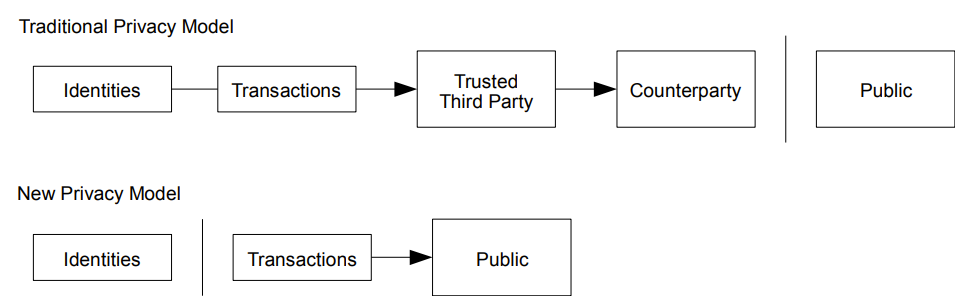
\includegraphics[width=\textwidth]{images/bitcoin-privacy.png}
\end{center}


\vfill

{\tiny Source: Satoshi Nakamoto. (2008). Bitcoin: A Peer-to-Peer Electronic Cash System. Retrieved from https://bitcoin.org/bitcoin.pdf}

\end{frame}

%------------------------------------------%
% Model
%------------------------------------------%

%\begin{frame}{Peer--to--peer Cannabis Traceability}
%
%\begin{itemize}
%
%\small
%
%\item {\bfseries Cryptographic proof} is used instead of {\itshape trust}.
%
%\vspace{1\baselineskip}
%
%\item {\bfseries Transparency} protects buyers and sellers from {\itshape fraud}.
%
%\vspace{1\baselineskip}
%
%\item {\bfseries Direct private transactions}, without having to {\itshape trust} counterparties or regulators.
%
%\end{itemize}
%
%\vfill
%
%{\tiny Source: Satoshi Nakamoto. (2008). Bitcoin: A Peer-to-Peer Electronic Cash System. Retrieved from https://bitcoin.org/bitcoin.pdf}
%
%\end{frame}


%------------------------------------------%
% Transactions
%------------------------------------------%

\begin{frame}{Cannabis Transactions}

\vspace{1\baselineskip}

\begin{center}
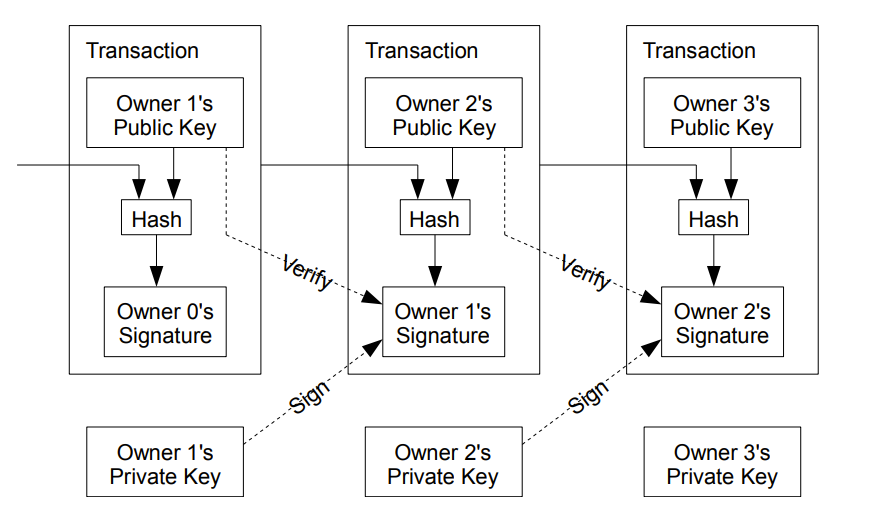
\includegraphics[width=\textwidth]{images/bitcoin-signing.png}
\end{center}

\vfill

{\tiny Source: Satoshi Nakamoto. (2008). Bitcoin: A Peer-to-Peer Electronic Cash System. Retrieved from https://bitcoin.org/bitcoin.pdf}

\end{frame}


%------------------------------------------%
% Blockchain
%------------------------------------------%

\begin{frame}{Cannabis Blockchain (CBC)}

\vspace{1\baselineskip}

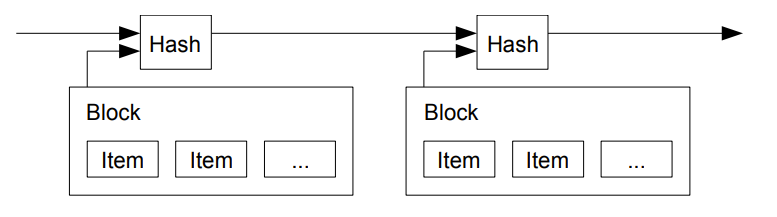
\includegraphics[width=\textwidth]{images/bitcoin-blockchain.png}

\vfill

{\tiny Source: Satoshi Nakamoto. (2008). Bitcoin: A Peer-to-Peer Electronic Cash System. Retrieved from https://bitcoin.org/bitcoin.pdf}

\end{frame}

%
%a hash of a block of items to be timestamped 
%
%wide publishing of the hash
%
%The timestamp proves that the data must have existed at the time
%
%additional timestamp reinforcing the ones before it
%
%Confirmations are nothing but just the number of blocks added after the block the transaction was added in


%------------------------------------------%
% Data
%------------------------------------------%


%------------------------------------------%
% Methodology
%------------------------------------------%



%------------------------------------------%
% Takeaway
%------------------------------------------%
\section{Takeaway}
\begin{frame}{}
\vspace{0.5\baselineskip}

% Thank you.
\begin{center}
\begin{minipage}{3.85in}

\includegraphics[width=.25in]{images/prayer.png} {\Large \textbf{Thank you for coming.}}\\[-0.75\baselineskip]
\end{minipage}
\end{center}

% Insights.
{\large Insight:}\\
\begin{itemize}
\vspace{0.5\baselineskip}
\item Build it and they will come.
\end{itemize}

\end{frame}


%------------------------------------------%
% Fin.
%------------------------------------------%
\end{document}
